\documentclass[11pt,a4paper,oneside]{article}

\usepackage[english,russian]{babel}
\usepackage[T2A]{fontenc}
\usepackage[utf8]{inputenc}
\usepackage[russian]{olymp}
\usepackage{hyperref}
\usepackage{graphicx}
\usepackage{expdlist}
\usepackage{mfpic}
\usepackage{amsmath}
\usepackage{amssymb}
\usepackage{comment}
\usepackage{listings}
\usepackage{epigraph}
\usepackage{url}
\usepackage{ulem}

\DeclareMathOperator{\nott}{not}

\begin{document}

\renewcommand{\t}[1]{\mbox{\texttt{#1}}}
\newcommand{\s}[1]{\mbox{``\t{#1}''}}
\newcommand{\eps}{\varepsilon}
\renewcommand{\phi}{\varphi}
\newcommand{\plainhat}{{\char 94}}

\newcommand{\Z}{\mathbb{Z}}
\newcommand{\w}[1]{``\t{#1}''}


\binoppenalty=10000
\relpenalty=10000

\createsection{\Note}{Комментарий}

\contest{Курс по предмету <<Структуры данных>>}{Сортировка слиянием во внешней памяти}{27 января 2018 года}

\textbf{Сортировка слиянием во внешней памяти}

\textbf{Филиппов Дмитрий, М4138}

Исходный код сортировки можно найти по адресу: \url{https://github.com/DimaPhil/external-merge-sort}.

\textbf{Описание задачи}

В задаче требуется реализовать сортировку данных, которые не помещаются в оперативную память и требуют сохранения на жесткий диск компьютера.
Сортировать можно разные объекты, но мы для упрощения рассмотрим здесь сортировку целых чисел и строк (однако с поддержкой сортировки и других объектов).

\textbf{Детали реализации}

Представим нашу задачу немного по-другому. Будем рассматривать данные как набор файлов, где размер каждого файла не очень большой (влезает в оперативную память). Тогда алгоритм сортировки будет выглядеть следующим образом: отсортируем каждый файл отдельно (это можно сделать in-memory), а затем смержим все файлы в один большой - это можно сделать $n$ указателями с дописыванием в итоговый файл.

В классе $utils/SortAndMergeUtils.scala$ представлена основная логика алгоритма~--- функция $sortAndMergeFiles$ получает на вход список файлов, которые надо отсортировать и смержить, а делает всю работу. В этой функции также добавлена логика разбиения файла на более маленькие, если его размер слишком большой~--- это сделано для того, чтобы код работал даже для списка файлов с большим объемом данных во избежание ручной работы, а также, чтобы алгоритм масштабировался под оставшееся количество оперативной памяти.

Для чтения и записи в файл используются классы $ReaderBuilder$, $WriterBuilder$, которые являются фабриками для ридеров и райтеров. Для данной задачи была использована одна из возможных реализация $Reader$ и $Writer$~--- $TextReader$ и $TextWriter$, которые используют $TextSerializer$ для чтения и записи данных. $TextSerializer$~--- обычный интерфейс с двумя методами $serialize$ и $deserialize$.

Вместе с этими интерфейсами реализация работы с файлами становится очень простой. Еще большой упрощает жизнь то, что $Reader$ реализует интерфейс $Iterator$, что позволяет работать с файлом как с обычным потоком данных.

Таким образом, алгоритм выглядит следующим образом:

\begin{itemize}
\item Разбить большие файлы на более маленькие, которые помещаются в оперативную память (оставшуюся);
\item Каждый маленький файл отсортировать
\item Начать сливать файлы
    \begin{itemize}
    \item Используем метод указателей
    \item На каждой итерации сливаем группы из $32$ файлов в один
    \item Продолжаем, уменьшив тем самым количество файлов в $32$ раза
    \end{itemize}
\item В результате получаем один файл, содержащий все данные~--- ответ
\end{itemize}

\textbf{Тестирование}

Для тестирования нашей реализации были проведены два набора тестов: первый~--- для строк, второй~--- для целых чисел. В каждом наборе тестов мы запускает $10^4$ подтестов, в каждом из которых сортируем данные из $100$ небольших файлов. После получения результата, сравниваем его с полученным руками (с сортировкой в оперативной памяти).

Также был проведен тест сортировки большого файла на 11Гб~--- но здесь после получения результата мы можем только проверить, что результат отсортирован. Однако, прохождение предыдущих тестов дает право утверждать, что все работает :)

\textbf{Время работы}

Для подсчета времени работы были проведены следующие тесты: 

\begin{itemize}
\item Мердж $10^4$ неотсортированных файлов по $10^5$ чисел~--- работает в среднем за $240$ секунд;
\item Мердж $10^4$ неотсортированных файлов по $10^4$ строк по $10$ символов~--- работает в среднем за $310$ секунд;
\item Сортировка одного большого файла на $10^9$ чисел (11 Гб)~--- около $40$ минут.
\end{itemize}

Приведем дополнительную информацию, показывающую зависимости некоторых величин:

Зависимость времени работы (сортировки $10^4$ файлов по $10^5$ чисел или $10^4$ строк по $10$ символов в каждом) в зависимости от количества чисел в одном файле (то есть чисел/строк, которые будут сортироваться в оперативной памяти). Количество чисел вычисляется по формуле $\min(10^7, freeMemory() / 4 / divisor)$, где $divisor$~--- параметр на оси графика. В рамках тестирования свободная оперативная память (freeMemory) была примерно равна 3Гб.

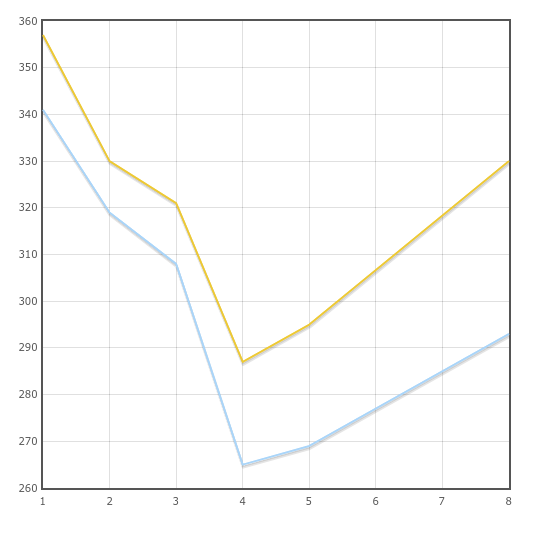
\includegraphics[natwidth=162bp,natheight=227bp]{img/02.png}

Здесь синией линией нарисован график для строк, желтой~--- для целых чисел.

Зависимость времени работы от количества сливаемых файлов (в основном коде использовали $32$, время замерялось на тесте из $10^4$ файлов по $10^5$ чисел, а также с $divisor = 4$):

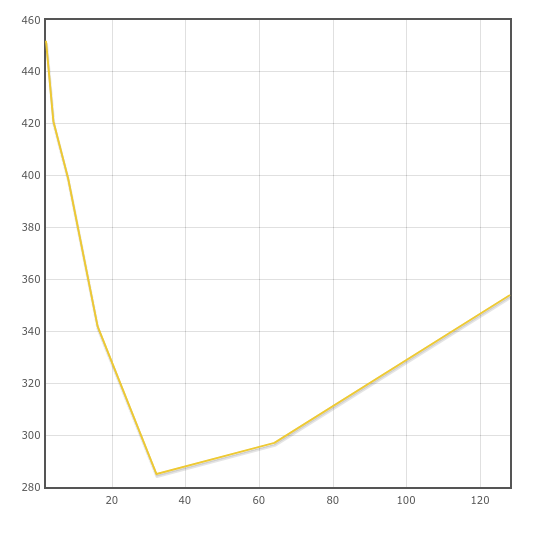
\includegraphics[natwidth=162bp,natheight=227bp]{img/01.png}

Зависимость времени работы от свободной оперативной памяти (результаты могут быть неточны, потому что $Runtime.getRuntime.freeMemory$ в Java может выдавать не совсем точные результаты из-за скачков памяти, а также размер свободной оперативной памяти может немного меняться в зависимости от других процессов):

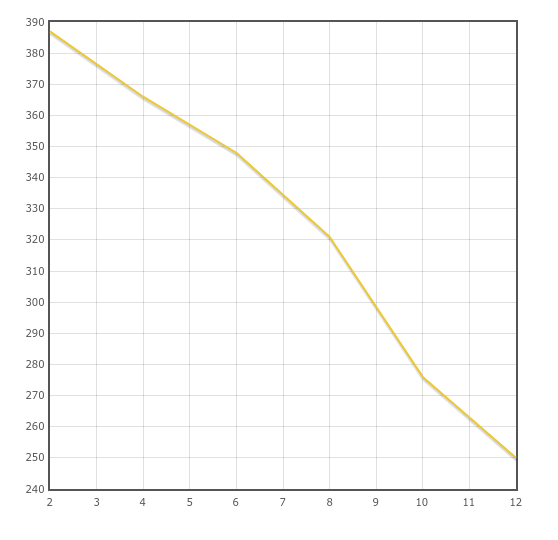
\includegraphics[natwidth=162bp,natheight=227bp]{img/03.png}


Возможно, результаты не идеальны, но по-моему вполне неплохие :)

\end{document}